\chapter{Literature Review}
\label{ch:lit}

\section{Outline}
This chapter reviews prior work on the focus areas of this thesis. Section~\ref{sec:lit-formats} covers how different sparse matrix formats are stored and
those how storage formats are chosen. Section~\ref{sec:lit-models} covers analytical operation-count and performance models for sparse kernels. Section~\ref{sec:lit-inputs} discusses the inputs used to evaluate sparse kernels. Section~\ref{sec:lit-accelerator} covers
sparse linear algebra on hardware accelerators, relevant to Chapter~\ref{ch:fpga}. Finally, Section~\ref{sec:lit-gaps} discusses how this thesis hopes
to address some of the gaps identified in the literature.

\section{Sparse Formats and Format Selection}
\label{sec:lit-formats}

\subsection{Formats beyond CSR, CSC, and COO}
Many different storage formats have been proposed to exploit certain matrices or hardware.
For hypersparse matrices, in which the number of non-zeros is very small relative to the dimension, CSR and CSC can waste space on the pointer arrays
that grow with their corresponding dimension. Buluc and Gilbert address this with their doubly compressed format (DCSC) that removes the empty-column
pointers and uses space proportional to the number of non-zeros \cite{bulucgilbert2008hypersparse}.
This is directly relevant to the Kronecker graphs studied in Chapter~\ref{ch:pact} and Chapter~\ref{ch:kron_taco}, where the number of non-zeros per row can be very small compared with
the dimension.

Other formats target specific hardware. Nvidia's Bell and Garland study SpMV on throughput-oriented processors, specifically GPUs \cite{bell2009implementing}.
Their work proposes their hybrid (HYB) format, which builds off of ELLPACK, first proposed in \cite{ellpack}.
In HYB, a regular part of the matrix is stored in ELLPACK format, which relies on consistent non-zeroes per row,
and any exceptional elements are stored in COO. For wide SIMD units, Kreutzer et al.\ propose SELL-$C$-$\sigma$, a SIMD-friendly
variant of sliced ELLPACK that combines ideas from GPU computing and vector processing, and show with fixed parameters that a single format can perform
very well across a Intel Sandy Bridge CPU, an Intel Xeon Phi, and an Nvidia Tesla K20 \cite{unified-format}.
Compressed sparse blocks (CSB) store a matrix as a grid of blocks so that both SpMV $Ax$ and sparse transpose $A^{T}x$ can
be computed efficiently in parallel \cite{bulucfineman2009csb}.

\subsection{Automated Format Selection}
Because no single format is best for all matrices, one area of research focuses on automating this choice. The Sparsity framework and its successor
OSKI tune SpMV with techniques such as register and cache blocking, symmetry, multiple vectors, variable-block and diagonal structure,
and reordering, selecting parameters using empirical measurements together with properties of the input matrix \cite{vuduc2003thesis,vuduc2005oski}.
SMAT gives programmers a single CSR-based interface and uses a decision tree learned from the features of 2,373 matrices in the University of Florida
collection to choose among CSR, DIA, ELL, and COO at run time \cite{li2013smat}. Sedaghati et al.\ show that no representation is uniformly best
on GPUs and train a classifier on matrix features to select one \cite{sedaghati2015automatic}.
Zhao et al.\ treat a matrix as an image and use a convolutional neural network for the same task \cite{zhao2018bridging}. Older investigations into automated
tuning research seemed to focus on analytical or empirical methods, while newer research has focused on machine learning techniques.

Most of these selection methods choose a single global format for a whole matrix, and further most target SpMV. One question studied in this thesis,
which pair of formats is best for a product of two sparse matrices, is not addressed by them. And indeed format selection
is a harder question for SpGEMM in which 2 matrices must be considered. Like the learned selectors above, this thesis chooses by measurement as well
as modeling, but it sweeps a controlled family of input kroneckers rather than a collection of unrelated matrices, see Section~\ref{sec:lit-inputs}).

\tikzset{
  tcell/.style={draw=black!70, minimum size=0.46cm, inner sep=0, font=\scriptsize},
  tname/.style={anchor=east, font=\scriptsize\ttfamily},
}
% \tarr{x}{y}{name}{comma-separated entries}: a labelled array of boxes
\newcommand{\tarr}[4]{%
  \node[tname] at ({#1-0.1},{#2}) {#3};
  \foreach \v [count=\i from 0] in {#4} {%
    \node[tcell] at ({#1+\i*0.46+0.23},{#2}) {\v};}}

\subsubsection{TACO.}
Compiler work approaches the problem of format selection from the other direction. Chou et al.\ give a unified description of formats
that lets a compiler generate kernels for arbitrary combinations \cite{taco_formats}, and TACO builds on this to generate tensor-algebra kernels
for mixed sparse and dense operands \cite{taco}. TACO is the mechanism used to produce the kernels in Chapter~\ref{ch:kron_taco}
and for reference in Chapter~\ref{ch:pact}. With this, format selection can be an experiment parameter to sweep across and identify crossovers.
The rest of this section explains both how TACO represents a matrix and its code generation.

\paragraph{Matrices as coordinate hierarchies.}
TACO takes a tensor expression in index notation together with a format for each operand, and generates imperative code from them \cite{taco}. For a matrix product, the
expression is $C_{ij} = \sum_k A_{ik}B_{kj}$. A format is described as a tree with one level per dimension, where each root-to-leaf path encodes the coordinates of one non-zero. Each level
has a \emph{level format} that says how its coordinates are stored. A \emph{dense} level stores only the dimension size and implicitly contains every coordinate. A \emph{compressed} level
stores only the coordinates present, in a \texttt{crd} array, plus a \texttt{pos} array giving where each parent's segment begins. A \emph{singleton} level stores one coordinate per parent
\cite{taco,taco_formats}. The 2018 extension also adds range, offset, and hashed levels, enough to express DIA, ELL, hash-map, and blocked formats \cite{taco_formats}, though this thesis will not examine these additional formats too closely.
The formats in this thesis are then compositions in TACO's language. CSR is a dense row level over a compressed column level; CSC is the same with the dimension order swapped; COO is a compressed, non-unique row level over a singleton column level. Figure~\ref{fig:taco-formats} shows one small matrix in each of these formats. Because a dense row level needs a \texttt{pos} entry per row
whether or not the row is empty, part of a format's cost scales with the dimension, not the non-zero count, which is the overhead DCSR removes.

\begin{figure}[t]
\centering
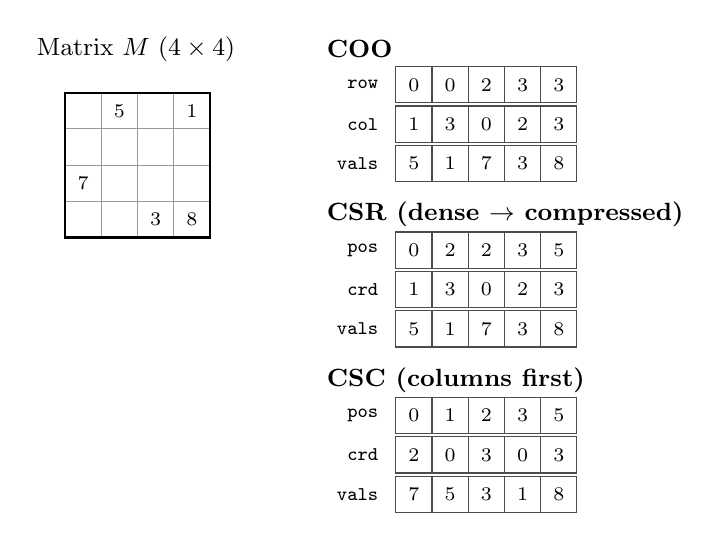
\begin{tikzpicture}[scale=1]
  \node[font=\small] at (0.9,0.55) {Matrix $M$ ($4\times 4$)};
  \draw[step=0.46cm, black!40, thin] (0,-1.84) grid (1.84,0);
  \draw[thick] (0,-1.84) rectangle (1.84,0);
  \foreach \r/\c/\v in {0/1/5, 0/3/1, 2/0/7, 3/2/3, 3/3/8}{%
    \node[font=\scriptsize] at ({\c*0.46+0.23},{-\r*0.46-0.23}) {\v};}
  \node[font=\small\bfseries, anchor=west] at (3.2,0.55) {COO};
  \tarr{4.2}{0.1}{row}{0,0,2,3,3}
  \tarr{4.2}{-0.4}{col}{1,3,0,2,3}
  \tarr{4.2}{-0.9}{vals}{5,1,7,3,8}
  \node[font=\small\bfseries, anchor=west] at (3.2,-1.55) {CSR (dense $\to$ compressed)};
  \tarr{4.2}{-2.0}{pos}{0,2,2,3,5}
  \tarr{4.2}{-2.5}{crd}{1,3,0,2,3}
  \tarr{4.2}{-3.0}{vals}{5,1,7,3,8}
  \node[font=\small\bfseries, anchor=west] at (3.2,-3.65) {CSC (columns first)};
  \tarr{4.2}{-4.1}{pos}{0,1,2,3,5}
  \tarr{4.2}{-4.6}{crd}{2,0,3,0,3}
  \tarr{4.2}{-5.1}{vals}{7,5,3,1,8}
\end{tikzpicture}
\caption{One matrix in three formats (indices from zero). In CSR, \texttt{pos[i]} to \texttt{pos[i+1]} delimits row $i$ in \texttt{crd}; row~1 is empty, so \texttt{pos[1]}$=$\texttt{pos[2]}. CSC is the same over columns. COO repeats the row coordinate per non-zero and has no \texttt{pos}.}
\label{fig:taco-formats}
\end{figure}

\paragraph{Format to Dataflow.}
The code generator reasons only about what each level can do. A dense level supports \emph{locate}, finding a coordinate's position directly; a compressed level can only be walked in order \cite{taco_formats}.
TACO orders the loops with an \emph{iteration graph}, so each operand is traversed top-down, and builds a \emph{merge lattice} for each index. A product needs the \emph{intersection} of its operands' coordinates. If neither operand supports locate, the
generated code co-iterates over both sorted coordinate lists, like the merge step of merge sort. If one does, it iterates the other's non-zeros and looks each up, reducing the cost from $O(\mathrm{nnz}(x)+\mathrm{nnz}(y))$ to just $O(\mathrm{nnz}(x))$ \cite{taco,taco_formats}.

\paragraph{Sparse $\times$ sparse products.}
In $A_{ij} = \sum_k B_{ik}C_{kj}$, the format pair therefore fixes how the sum over $k$ is organized.
With $B$ and $C$ both CSR, the order $i,k,j$ works and the dense row level of $C$ lets the code locate row $k$, giving the row-wise (Gustavson) dataflow. With $B$ in CSC and $C$ in CSR, both have $k$ at the top, so $k$ is the outermost loop, giving the outer-product dataflow.
With $B$ in CSR and $C$ in CSC, $k$ is innermost and two sparse lists are intersected per output element, giving the inner-product dataflow. Choosing formats thus largely chooses the dataflow, so the sweep over format pairs in Chapter~\ref{ch:kron_taco} is also a sweep over algorithms.

\paragraph{Limits.}
Blocked formats are expressible with fixed-size dense levels, so block sizes must be uniform \cite{taco_formats}. As well blocks of differing format are inexpressible.
The published evaluation covers SpMV, sparse $\times$ dense multiplication, addition, and tensor kernels, single-threaded, on matrices up to about $1.3\mathrm{M}\times 1.3\mathrm{M}$ \cite{taco_formats}, so sparse $\times$ sparse products at the scales of Chapter~\ref{ch:kron_taco} are beyond what those papers measure.

\subsection{Heterogeneity within a matrix}
A few approaches already store different parts of a matrix differently. HYB, as mentioned before, divides a matrix between
two formats \cite{bell2009implementing}. Vuduc and Moon split modify the traditional Block Compressed Sparse Row (BCSR) and propose Unaligned BSCR (UBSCR), in which a matrix is split into parts with different register block sizes to exploit variable block structure \cite{vuduc2005vbr}.

The closest prior work to the per-block pipeline of Chapter~\ref{ch:pact} that I am aware of is TileSpMV for GPUs, which
partitions a matrix into tiles, implements seven SpMV kernels for tiles stored in different formats, and selects the format
and algorithm for each tile based on its local sparsity structure \cite{niu2021tilespmv}. This was extended to SpGEMM in TileSpGEMM, which adapts the
tiling idea of dense matrix multiplication: it splits both matrices into fixed-size sparse tiles, so that work per tile is easier to balance and accumulate.
It is evaluated on 142 square matrices against four GPU libraries (cuSPARSE, bhSPARSE, NSPARSE, and spECK) and is reported to be faster than the best of
them, spECK, on 94 of the 142 \cite{niu2022tilespgemm}. TileSpGEMM is the closest SpGEMM analogue to the blocking of Chapter~\ref{ch:pact}, but it targets GPUs,
uses one sparse block format/representation rather than selecting among many formats, and is not concerned with choosing CPU-side format pairs.

Table~\ref{tab:lit-formats} summarizes how these approaches compare.

\begin{table}[h]
\centering
\small
\begin{tabular}{p{3.0cm}p{1.6cm}p{2.6cm}p{4.6cm}}
\hline
\textbf{Work} & \textbf{Kernel} & \textbf{Granularity} & \textbf{Selection} \\
\hline
Sparsity/OSKI \cite{vuduc2003thesis} & SpMV & whole matrix & empirical profile plus heuristic \\
SMAT \cite{li2013smat} & SpMV & whole matrix & learned model \\
Sedaghati et al.\ \cite{sedaghati2015automatic} & SpMV & whole matrix & learned classifier \\
Zhao et al.\ \cite{zhao2018bridging} & SpMV & whole matrix & convolutional network \\
TileSpMV \cite{niu2021tilespmv} & SpMV & per tile & per-tile selection method \\
TileSpGEMM \cite{niu2022tilespgemm} & SpGEMM & per tile & none, single format \\
\hline
\end{tabular}
\caption{Format-selection approaches compared by kernel, granularity, and selection method.}
\label{tab:lit-formats}
\end{table}

\section{Motivating Flop and Memory-Operation Models}
\label{sec:lit-models}

For each pair of operand formats, Chapter~\ref{ch:pact} derives the number of floating point operations and memory operations the
respective SpGEMM kernel performs. This section motivates why such counts are a reasonable thing to model, what related models exist, and their limits.

\subsection{Operation Counts}
Sparse kernels often do little arithmetic per byte moved. Additionally, the work they do end up doing depends on the structure of the inputs,
not just on their dimensions. The roofline model relates attainable performance to the number of operations performed per byte of memory traffic and to
the hardware's compute and bandwidth ceilings \cite{roofline}. It is the standard model for asking whether a kernel is limited by memory or
by compute. Applying it to a given SpGEMM requires knowing how many operations and how many memory accesses the chosen algorithm and formats perform, see Table~\ref{tab:formulas}.

Operation counts also appear inside algorithm analyses. The sequential hypersparse kernel of Buluc and Gilbert has a running time that depends on the number of non-empty columns of one operand, the number of non-empty rows of the other, and the number of scalar multiplications. It is therefore independent of the matrix dimension, which is one reason the outer-product formulation suits hypersparse inputs \cite{bulucgilbert2010highly}, as we will see in Chapter~\ref{ch:kron_taco}. That bound is stated for one algorithm and one format, it does not compare formats.

\subsection{Using operation counts for prediction}
Two bodies of work suggest that quantities derived from operation counts predict which implementation is best. Nagasaka et al.\ find that the best SpGEMM algorithm on multicore and many-core processors varies with matrix size, sparsity, the compression factor of the product, and the operation being performed, and they distill their measurements into a recipe for choosing among hash-based, heap-based, and library implementations \cite{nagasaka2018highperformance}. Looking into the field of custom accelerators, Flexagon argues that different workloads favor different dataflows depending on features of the kernel such as its dimensions, sparsity pattern, and sparsity degree, and builds hardware that runs each computation with the dataflow that best suits it \cite{munoz2023flexagon}.

Many of these lines of research choose between algorithms or dataflows. But as established in Chapter~\ref{ch:background}, format and dataflow are
very tightly coupled.

\subsection{Limits of operation counts}
Counts describe what the algorithm asks the machine to do, not what the machine does. They do not capture cache behavior, branch misprediction, page faults and first-touch costs, etc. Hardware performance counters measure these effects directly, but they are often not exact. On eleven x86-64 implementations, events that should be deterministic, such as retired instructions, vary from run to run and overcount, with hardware interrupts and page faults among the sources \cite{weaver2013nondeterminism}. Counts and counters are therefore complementary. We will find in Chapter~\ref{ch:pact} that the operation-count formulae predict runtime poorly, and Chapter~\ref{ch:kron_taco} uses cache-miss, branch-misprediction, and page-fault counters to hopefully examine and explain the discrepancy.

\section{Benchmark Inputs for Sparse Kernels}
\label{sec:lit-inputs}

\subsection{Collections of real matrices}
Evaluations of sparse kernels commonly draw on the SuiteSparse Matrix Collection \cite{davis2011suitesparse,kolodziej2019suitesparse}, which includes matrices from the SNAP network datasets \cite{leskovec2014snap,leskovec2016snaplib}. Studies typically report results per matrix across large sets. SMAT is trained on features of 2,373 matrices \cite{li2013smat}, and TileSpGEMM is evaluated on 142 square matrices, each requiring at least one billion floating-point operations for one SpGEMM \cite{niu2022tilespgemm}. Such evaluations are broad, but they do have a structural limitation: every matrix differs from every other in size, density, and structure at once. When a method wins on one matrix and loses on another, the data cannot easily say which of the three properties is responsible. Each matrix is a single point, and can not point us to a interpolatable trend.

\subsection{Synthetic generators}
Synthetic generators offer a bit more control. The R-MAT model recursively subdivides an adjacency matrix according to a small set of probabilities to produce graphs with power-law degree distributions \cite{chakrabarti2004rmat}. Kronecker graph models generate self-similar graphs by repeated Kronecker products of a small initiator matrix and can be fitted to real networks \cite{kronecker,moez}. Because the number of repetitions is a free parameter, a single fitted model can be generated at many scales, so that structure is held approximately fixed while size varies.

\section{Hardware Acceleration for Sparse Computations}
\label{sec:lit-accelerator}

\subsection{SpGEMM accelerators and dataflows}
Gustavson's row-wise algorithm is one classical formulation of sparse matrix multiplication \cite{gustavson1978} as it requires no intersection operation of non-zeroes. Recent accelerator work revolves around choosing among inner-product, outer-product, and row-wise dataflows. OuterSPACE pursues outer products \cite{pal2018outerspace}. SpArch observes that the outer product suffers from poor output locality because of the numerous partial product matrices it generates, and addresses this with on-chip merging, a condensed matrix representation that reduces the number of partial matrices, a Huffman-tree merge scheduler, and a row prefetcher \cite{zhang2020sparch}. MatRaptor adopts the row-wise product and introduces a storage format, C2SR, that lets parallel compute engines access sparse data in a streaming way \cite{srivastava2020matraptor}. Gamma builds on Gustavson's algorithm for GPU-like architectures \cite{zhang2021gamma}. Flexagon is a reconfigurable accelerator that supports all three dataflows \cite{munoz2023flexagon}. Two themes recur: the dataflow determines which operand is reused and which output is accumulated, and accelerator designers have found it worthwhile to design the storage format together with the dataflow, as MatRaptor does. This parallels the format-pair question of this thesis, at the hardware level.

\subsection{FPGA implementations}
FPGA implementations of SpMV have been studied extensively because the kernel is dominated by irregular memory access. Fowers et al.\ propose a sparse matrix encoding that exposes parallelism across rows together with a banked vector buffer, and report competitive performance against CPUs and GPUs at lower power \cite{fowers2014fpga}. Hosseinabady and Nunez-Yanez describe a streaming dataflow engine for SpMV on embedded FPGAs built with high-level synthesis, combining loop pipelining, dataflow graphs, and data streaming to use most of the available memory bandwidth; they report about $3.25\times$ the performance of embedded GPUs on small and medium matrices and about $8.9\times$ better energy efficiency than the embedded CPU and GPU \cite{fpga-stream}. This is the design style used in Chapter~\ref{ch:fpga}. Work on irregular matrices addresses load imbalance \cite{overcoming-irreg}, and CPU work selects among hybrid formats adaptively for SpMV \cite{hybrid_format}.

\section{Gaps Identified}
\label{sec:lit-gaps}

Taken together, the literature reviewed suggests three points that this thesis tries to address.
\begin{enumerate}
  \item \textbf{Evaluations are made at single points.} Collections of real matrices vary size, density, and structure together, so the dependence of the best choice on any one of them cannot be separated. Kronecker graphs fitted to real networks can be generated at many scales, and Chapter~\ref{ch:kron_taco} sweeps them to show how the best format pair changes as size grows.
  \item \textbf{Format selection is studied mostly for SpMV and mostly per matrix.} Selection of format \emph{pairs} for SpGEMM appears less explored. Chapter~\ref{ch:pact} contributes flop and memory-operation formulae for sixteen format pairs, and Chapter~\ref{ch:kron_taco} compares the pairs by measurement and with hardware counters.
  \item \textbf{Heterogeneous formats within one matrix have been attempted for SpMV but their SpGEMM cost is less documented.} Chapter~\ref{ch:pact} presents a per-block selection pipeline for SpGEMM and reports that it unfortunately did not pay off along with an analysis of why.
\end{enumerate}
